\documentclass[../main.tex]{subfiles}
\begin{document}

\chapter{Experiments and Discussion}\label{exp:chap}

Having defined preliminaries and the implementation for our approach to the problem of GMG, we now
turn to the experiments to evaluate our methodology and an analysis of the respective results.

\section{GCBC's Instruction Following Capabilities}

We initially focus on the verification of our approach with a specific focus on GCBC's ability to
follow instructions. We strive to determine if our model's choices are justifiable, if it can handle
somewhat realistic scenarios, and if its capabilities are up to par.

\subsection{The CALVIN dataset}

Introduced by \citet{mees_calvin_2022}, CALVIN (\textbf{C}omposing \textbf{A}ctions from
\textbf{L}anguage and \textbf{Vi}sio\textbf{n}) is a benchmark originally intended for training and
evaluating models on long-horizon language-conditioned tasks. That is, a multi-task set of 34 SDM tasks where the expected interaction sequence is considerably long (up to 240 steps, due to task
chaining) and the tasks are specified via language. The benchmark consists of, among other things,
an environment and a dataset.

\begin{figure}[t]
	\centering
	\setlength{\tabcolsep}{2pt}
	\begin{tabular}{c c c}
		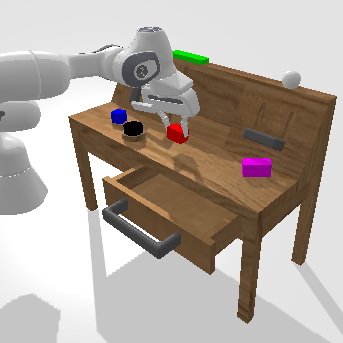
\includegraphics[width=0.32\linewidth]{figures/calvin/scene.png}        &
		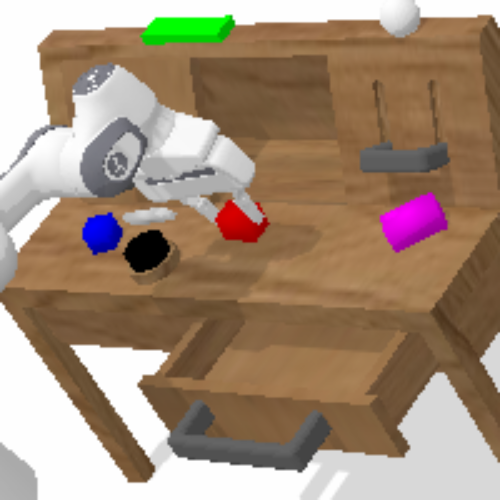
\includegraphics[width=0.32\linewidth]{figures/calvin/rgb_static.png}   &
		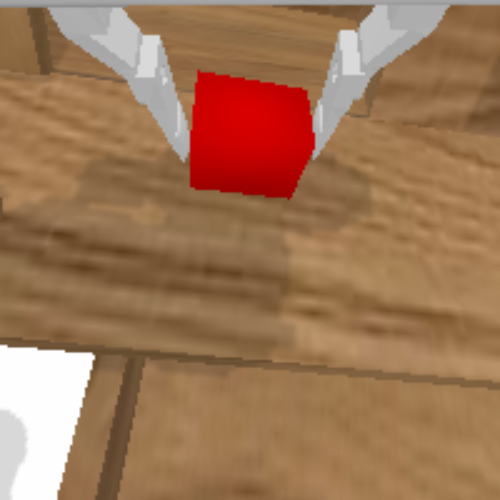
\includegraphics[width=0.32\linewidth]{figures/calvin/rgb_gripper.png}    \\
		
\includegraphics[width=0.32\linewidth]{figures/calvin/tactile.png}      &
		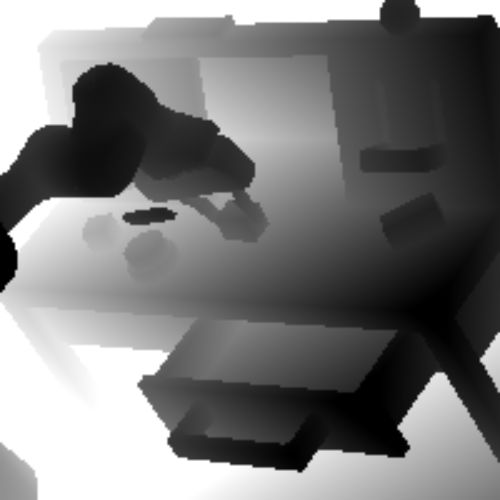
\includegraphics[width=0.32\linewidth]{figures/calvin/depth_static.png} &
		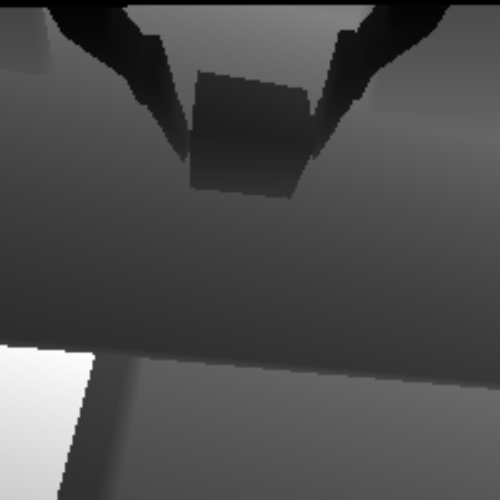
\includegraphics[width=0.32\linewidth]{figures/calvin/depth_gripper.png}
	\end{tabular}
	\caption[The available perceptive state in the CALVIN environment.]{An overview of
		the perceptive state in the CALVIN environment. Top, left to right: scene, static and gripper RGB
		images. Bottom, left to right: tactile, static depth, gripper depth. Figure courtesy
		of~\citet{mees_calvin_2022}}
	\label{fig:calvin}
\end{figure}

\begin{table}[t]
	\centering
	\caption[The CALVIN 15-D proprioceptive state and 7-D action vectors.]{The CALVIN 15-D
		proprioceptive state and 7-D action vectors. \textbf{Bold} indicates that these dimensions are
		present in both proprioceptive state and action space. In case of actions, these can either be
		``static'' (relative to the world frame) or ``relative'' (displacements relative to the
		gripper frame). In case of state, this is always static.}
	\label{tab:calvin-proprio}
	\begin{tabular}{@{}rl@{}}
		\toprule
		Dimension(s) & Description                                                             \\ \midrule
		\textbf{0-2} & \textbf{TCP $(x, y, z)$ coordinates}                                    \\
		\textbf{3-5} & \textbf{TCP $(x, y, z)$ euler angle coordinates}                        \\
		6            & Gripper opening width (meters)                                          \\
		7-13         & Robotic arm joint state (rad)                                           \\
		\textbf{14}  & \textbf{Binary gripper action ($\text{close} = -1$, $\text{open} = 1$)} \\ \bottomrule
	\end{tabular}
\end{table}

\begin{table}[t]
	\centering
	\caption[The 34 tasks of the CALVIN environment]{The 34 tasks of the CALVIN environment and an
		example natural language annotation. Some tasks are grouped together due to similarity. We note
		the group sizes with the numbers in the parentheses.}
	\label{tab:calvin-tasks}
	\footnotesize
	\begin{tabular}{@{}ll@{}}
		\toprule
		Task                                 & Example annotation                                    \\ \midrule
		Rotate red/blue/pink block right (3) & ``turn the red block right''                          \\
		Rotate red/blue/pink block left (3)  & ``turn the blue block left''                          \\
		Push red/blue/pink block right (3)   & ``push right the pink block''                         \\
		Push red/blue/pink block left (3)    & ``push left the red block''                           \\
		Move slider left/right (2)           & ``slide the door to the left''                        \\
		Open/close drawer (2)                & ``go open the drawer''                                \\
		Lift red/blue/pink block table (3)   & ``pick up the red block''                             \\
		Lift red/blue/pink block slider (3)  & ``lift red block from slider''                        \\
		Lift red/blue/pink block drawer (3)  & ``lift blue block from drawer'                        \\
		Place in slider/drawer (2)           & ``put the grasped object in the slider''              \\
		Push into drawer (1)                 & ``push the block into thedrawer''                     \\
		Stack blocks (1)                     & ``stack blocks on top of each other''                 \\
		Unstack blocks (1)                   & ``collapse the stacked blocks''                       \\
		Turn on/off light bulb (2)           & ``toggle the light switch to turn on the light bulb'' \\
		Turn on/off LED (2)                  & ``push the button to turn off the green light''       \\ \bottomrule
	\end{tabular}
\end{table}

The environment simulates a 7-DOF\footnote{\textit{scilicet}: degrees of freedom.} Franka Emika
Panda robot arm~\citep{haddadin_franka_2022} interacting with three rectangular objects of different
colors and shapes on a desk. The desk additionally features a sliding door and drawer that can both
be opened and closed. Finally, a button and switch can be used to activate a green light and light
bulb respectively. The observation space consists of RGBD\footnote{\textit{scilicet}: red, green,
	blue and depth channels.} images from a static camera as well as from a camera mounted to the
robotic arm's gripper, with dimensionality $200 \times 200$ and $84 \times 84$ respectively.
A vision-based sensor additionally provides images of shape $160 \times 160 \times 6$ for tactile
information at the gripper. Figure~\ref{fig:calvin} presents an overview of the perceived state.
Finally the proprioceptive state is also available in the form of a 15-dimensional vector describing
the TCP\footnote{\textit{scilicet}: tool center tip} position and orientation, as well as gripper
state and arm joint states.  For acting, models operating in the CALVIN environment sample from
a continuous 7-dimensional action space describing the position and orientation of the TCP and
gripper activation. Table~\ref{tab:calvin-proprio} provides an overview of what each dimension of
the proprioceptive state and action vectors corresponds to. The authors define 34 different tasks
that can be performed in the environment and can be labelled with natural language instructions,
which we present in Table~\ref{tab:calvin-tasks}. The environment comes with an oracle that can
check for the completion of a task in a given sequence of steps, as defined by specific changes of
the state between the initial and final steps in the sequence. The environment can take any of four
configurations A, B, C, and D, which are structurally identical but present some differences in e.g.
table colour.

The CALVIN \emph{dataset} consists of $\sim$2.2M demonstrations across the four environment
configurations. This is largely composed of ``unstructured'' demonstrations, recordings of
exploratory and even random expert interactions with the environment, equivalent to the ``play''
data described in the previous chapter. The authors then crowd-source over 400 natural language
instructions describing the 34 tasks, and procedurally label 1\% of the demonstrations with these
instructions when possible, i.e. when they find that a given demonstration solves one of the 34
tasks. For our work, we restrict our attention to the D configuration of the environment, equivalent
to $\sim$700K demonstrations. We choose to validate our approach using the CALVIN benchmark due to
its more realistic and challenging nature. We expect that if our implementations successfully learn
an instructable policy for such a benchmark, then they should be straightforward to apply to more
easily configurable setups. Additionally, we believe demonstrating applicability to CALVIN could be
a good indicator of the soundness and/or generalizability of our approach.


\subsection{CLIPT}

We use CLIPT as the specification encoder of our GCBC solution. As previously mentioned, we train
CLIPT separately from GCBC. We do this because we approach the problem from the recently prevalent
perspective of utilizing representations from pre-trained foundation models for applications on
downstream tasks. We take this approach because we expect future solutions to follow this trend, at
least in the short-term. Under this framework, we treat CLIPT as a stand-in for such a foundation
model, and GCBC as the beneficiary of the representations.

\subsubsection{Training details}\label{exp:sec:clipt-train}

We train CLIPT on the subset of CALVIN that is language-annotated, sampling only the start and end
state of each trajectory. This amounts to a total of 5124 training samples, and 1011 validation
samples, each consisting of two images and the natural language instruction. We use the Adam
optimizer~\citep{kingma_adam_2015} with a learning rate of $5 \times 10^{-5}$. For both training
phases, we train for a total of 50 epochs, allowing for early stopping if the validation loss does
not improve for 3 epochs, and use the checkpoint with the best validation loss. We use LAION's
"CLIP-ViT-L-14-laion2B-s32B-b82K" checkpoint of OpenCLIP~\citep{ilharco_openclip_2021} throughout
our work. This is a version of CLIP relying on an L-14 variant of the visual transformer (ViT)
architecture~\citep{dosovitskiy_image_2022} for the vision encoder, pretrained on the 2 billion pair
subset of the LAION-5B dataset~\citep{schuhmann_laion-5b_2022}.

\subsubsection{CLIPT sanity checks}

We perform a number\footnote{we outline our two main checks here, and present our other CLIPT sanity
	checks in Appendix~\ref{app:clipt-sanity}.}of sanity checks on the soundness of our CLIPT design.
Our main concern is whether CLIPT is making use of the crucial information contained in the second
half of its input. We hold this concern due to the fact that the first half of the input to
$\text{MLP}_\text{vis}$ and $\text{MLP}_\text{txt}$ is the same, namely the CLIP representation of
start state, $\vect{v}_s$. Given that CLIPT is trained contrastively, the MLP encoders could be
pressured into simply relying on the first half of the input while ignoring the second half while
constructing representations, as this would contain sufficient information for matching true pairs
of goal representations.

The first check we perform consists in setting the second half of the input to a 0-valued vector at
inference time, and evaluating whether this affects performance. We expect that if CLIPT is indeed
ignoring the second half of its input, then masking it in this way should not affect performance. To
perform our check, we operate on the validation split of the CALVIN dataset, sampling 256
trajectories for which we compute pairs of visual and textual trajectory representations using
CLIPT's $\text{MLP}_\text{vis}$ and $\text{MLP}_\text{txt}$ respectively. We then compute the cosine
similarity between every possible pairing, for a total of $256^2$ similarity scores. We then
evaluate in two ways. First, we visualize the scores in a similarity matrix. Second, we compute the
\emph{top-$k$ accuracy} of CLIPT, that is, the proportion of times that the correctly paired visual
representation is in the top-$k$ visual representations ranked by similarity to a given textual
representation. We perform this evaluation with normal CLIPT representations as a baseline, and with
masked representations as described above as an ablation and compare. Figure~\ref{fig:clipt-masked}
and the first two rows of Table~\ref{tab:clipt-eval} present the results of this first check. We see
that the diagonal disappears in the ablation, and that the top-$k$ accuracy metric faces relative
drops between -60\% and -90\%. Based on these results, we had some evidence suggesting that CLIPT
was indeed behaving as intended.

\begin{figure}[t]
	\centering
	\includegraphics[width=\textwidth]{figures/sim_matrices}
	\caption[Similarity matrices of baseline and masked CLIPT]{Similarity matrices of the baseline
		(left) and masked (right) representations from CLIPT. The ideal matrix should display a peak in
		similarity along the diagonal.}
	\label{fig:clipt-masked}
\end{figure}

\begin{table}[t]
	\centering
	\caption[Top-$k$ accuracy of CLIPT]{Top-$k$ accuracy of CLIPT. The first two rows show the
		statistics when using normal and masked representations, on CLIPT trained over two phases. The
		final two rows shows the statistics of correctly paired (Sing.Ph.) and randomly paired (Rand.P.)
		representations when training in a single phase.}
	\label{tab:clipt-eval}
	\begin{tabular}{@{}rcccccc@{}}
		\toprule[1.5pt]
		\textbf{Top-$k$ accuracy} & $k=1$ & $k=3$ & $k=5$ & $k=10$ & $k=20$ & $k=50$ \\ \midrule
		\textbf{Baseline Repr.s}  & 0.238 & 0.457 & 0.570 & 0.773  & 0.906  & 0.973  \\
		\textbf{Masked Repr.s}    & 0.016 & 0.031 & 0.047 & 0.082  & 0.176  & 0.363  \\ \midrule
		\textbf{Sing.Ph. Repr.s}  & 1.000 & 1.000 & 1.000 & 1.000  & 1.000  & 1.000  \\
		\textbf{Rand.P. Repr.s}   & 1.000 & 1.000 & 1.000 & 1.000  & 1.000  & 1.000  \\
		\bottomrule[1.5pt]
	\end{tabular}
\end{table}

We perform another check, more closely concerned in verifying the necessity of training in two
phases. We posit that training in a single phase, with both $\text{MLP}_\text{vis}$ and
$\text{MLP}_\text{txt}$ instantiated from the start, would indeed result in CLIPT learning to ignore
the second half of its input due to the shared first half of the input across visual and textual
representations. To verify this, we train a version of CLIPT in a single phase as described above
and repeat the top-$k$ accuracy evaluation and treat this as a baseline. We then repeat training on
a new instance of CLIPT, but pair the representations randomly, treating this as an ablation. More
specifically, during training, we use the same start state first halves of the representations used
for the baseline, but then sample random instructions for a given end state, rather than the correct
pairing. During testing, we repeat the top-$k$ accuracy evaluation using appropriately paired
representations. If CLIPT is indeed ignoring the second half, we would expect performance to be
unchanged between baseline and ablation. We report the result of this experiment in the final two
rows of Table~\ref{tab:clipt-eval}. We note that in both cases we achieve perfect top-k accuracy,
which we explain as only possible if the model learns to ignore the second half and learn to match
the (identical) first halves of the input vectors. We therefore conclude that our two-phase training
setup is indeed necessary.

\subsection{GCBC}

We turn our attention to our GCBC implementation. Here, we are concerned with determining whether an
acceptable performance is achievable and whether a gap forms between the performance when
conditioned on visual trajectories and when conditioned on textual trajectories.

\subsubsection{Training details}

We train GCBC on the play-data trajectories comprising the CALVIN dataset, equivalent to
$\sim$740\,000 training samples. Each sample consists of a sequence of states and actions,
corresponding to the trajectory of a demonstration interacting with the environment and optionally
a language annotation. The sequences are of variable length, ranging between 28 and 32 frames. We
train for 10 epochs, conditioning on visual trajectory representations from CLIPT. We use the
checkpoint from the final epoch for evaluation. We once again use the Adam
optimizer~\citep{kingma_adam_2015}, with a learning rate of $5 \times 10^-5$. Because the action
space in CALVIN is a multivariate continuous action space, we use the DLML-based continuous actor
module described in Section~\ref{meth:sec:actor-modules:continuous}.

\subsubsection{Evaluation details and results}\label{exp:sec:gmg-eval}

We evaluate our GCBC checkpoints by leveraging the oracle included in the CALVIN environment.
Specifically, for each of the 34 tasks in our environment we recover 100 valid starting states from
our test split. For each of the 100 start states, we condition our policy to complete the task and
let it interact with the environment for a maximum of 240 steps, performing a ``rollout''. We reset
the GRU hidden state every 28 steps. At each step, we use the oracle to verify whether the task has
been completed. If the task is completed within the 240 steps, we deem this interaction a success.
We measure the success rate over the 100 rollouts for each task. To assess the gap between visual
trajectory representations (on which the policy is trained) and textual trajectory representations
(which we use at inference time), we perform this evaluation twice: once conditioning on textual
trajectory representations, and the other conditioning on visual trajectory representations.

\begin{figure}[t]
	\centering
	\includegraphics[width=\textwidth]{figures/gcbc_calvin/gcbc_resets}
	\caption[GCBC success rate on the CALVIN dataset]{GCBC success rate on the CALVIN dataset.}
	\label{fig:gcbc-calvin-res}
\end{figure}

\begin{table}[tb]
	\centering
	\caption[GCBC success rate on the CALVIN dataset]{Summary evaluation statistics of the GCBC
		experiments on CALVIN. The first two rows present the success rate (SR) statistics for our
		reference checkpoint, trained on CLIPT-2P representations and evaluated with context resets. The
		following two rows present the SR statistics when we have no context resets (NCR) during
		evaluation. The final row presents the SR statistics when conditioning on textual trajectory
		representations from CLIPT-1P, i.e. directly from CLIP's text encoder. Statistics computed across the 34-task set. Multiple seeds were not run due to computational limitations.}
	\label{tab:gcbc-calvin-res}
	\begin{tabular}{@{}rccccc@{}}
		\toprule[1.5pt]
		\textbf{}                    & \textbf{mean}    & \textbf{median} & \textbf{min} & \textbf{max}
		                             & \textbf{std err}                                                        \\ \midrule
		\textbf{Text. SR (ref)}      & 0.41             & 0.27            & 0.05         & 0.97         & 0.05 \\
		\textbf{Vis. SR (ref)}       & 0.36             & 0.32            & 0.08         & 0.79
		                             & 0.04
		\\ \midrule[0.05pt]
		\textbf{Text. SR (NCR)}      & 0.28             & 0.15            & 0.04         & 0.92         & 0.04 \\
		\textbf{Vis. SR (NCR)}       & 0.25             & 0.15            & 0.01         & 0.82
		                             & 0.04                                                                    \\ \midrule[0.05pt]
		\textbf{Text. SR (CLIPT-1P)} & 0.16             & 0.14            & 0.00         & 0.69
		                             & 0.03                                                                    \\ \bottomrule[1.5pt]
	\end{tabular}
\end{table}


Figure~\ref{fig:gcbc-calvin-res} and the first two rows of Table~\ref{tab:gcbc-calvin-res} summarize
the results of the evaluation of GCBC on the CALVIN dataset. With textual trajectories, we note
a mean success rate of 0.41 and a median success rate of 0.27, going as high as 0.97 for some tasks
and as low as 0.05 for others. Prior work achieved a better performance of around
0.647~\citep{mees_calvin_2022}. Direct comparisons are perhaps inappropriate however. We trained for
less time due to computational limits and relied on a slightly different architecture with the use
of CLIPT, training exclusively on visual goals rather than both vision and language. For context,
we perform an additional evaluation to test whether the policy takes the goal conditioning into
account or simply relies on the current state. We condition on random vectors rather than the
representations from CLIPT, and find that the mean and median success rate drop to
0.09 and 0.04 respectively. There is a gap between the performance on visual and textual
trajectories, and surprisingly the policy appears to perform better with textual trajectory
representations than on visual trajectory representations, despite being trained on the latter.
This gap however, is relatively small. We reserve further discussion and analysis of the results
to Section~\ref{exp:sec:discussion}.

\subsubsection{Other experiments and results}

We perform additional experiments to better understand the impact of design choices made in GCBC on
the performance of the policy. We first inspect the impact of context resets during inference. We do
this by repeating evaluation without context resets, and comparing the performance to the baseline
where we reset the hidden state every 28 steps. We report our findings in the rows labeled ``NCR''
in Table~\ref{tab:gcbc-calvin-res}. We can see that omitting context resets during inference results
in a clear drop in performance by around 30\%, with the mean success rate dropping from 0.41 to 0.28
when conditioning on textual trajectory representations, and from 0.36 to 0.25 when conditioning on
visual trajectory representations. Similar drops are also noted on the median values. The gap
between visual and textual performance remains small however. We see that, perhaps unsurprisingly,
our GRU-based architecture is sensitive to the sequence lengths longer than what it was trained on,
but that this has no effect on whether it handles textual and visual trajectory representations
differently.

To better assess the importance of our two-phase training, we repeat evaluation using the CLIPT
checkpoint just before the start of the second phase of training. This is when
$\text{MLP}_\text{vis}$ has been trained, but $\text{MLP}_\text{txt}$ does not exist yet, such that
the textual trajectory representations come directly from CLIP's text encoder. We report our
findings in the final row of Table~\ref{tab:gcbc-calvin-res}. Note that the performance when
conditioning on visual trajectory representations is unchanged, so we refer to the second row of the
table for that. We see that the gap in performance when conditioning on textual trajectories as
opposed to visual trajectories is now large, with a mean SR of $0.16 \pm 0.03$ when
conditioning on natural language as opposed to a mean SR of $0.36 \pm 0.04$  when conditioning on
visual goals. This underlines the importance of our two-phase training of CLIPT in allowing us to
train on visual trajectory representations and swapping these for textual trajectory representations
at inference time.

\section{Addressing goal misgeneralization}\label{exp:sec:gmg}

We now turn to the problem of addressing GMG. We rely on a more manageable environment and dataset
platform, and construct a toy-scenario for observing the phenomenon.

\subsection{The BabyAI platform}

Introduced by \citet{chevalier-boisvert_babyai_2022}, BabyAI is a platform originally designed for
the study of grounded language learning via human-in-the-loop experiments. It consists of
a collection of 19 grid-world environments\footnote{Also referred to as ``levels''.} of various
difficulty, based on the MiniGrid and Gymnasium libraries~\citep{chevalier-boisvert_minigrid_2023,
	towers_gymnasium_2023, brockman_openai_2016}. Each environment corresponds to a class of tasks, such
as moving to an object, placing an object next to another, unlocking doors and more. Distractors,
i.e.~ objects unrelated to the task at hand, may be placed in the environment to complicate the
completion of the task. Any instantiation of a BabyAI environment scene will come with an associated
language instruction in ``Baby Language'', a combinatorially rich subset of English unambiguously
understood by humans. We present example Baby Language instructions in Figure~\ref{fig:baby-lang}
and a visual example of the environment state in Figure~\ref{fig:gmg-cc-example}. The environment
state is represented as a $7 \times 7 \times 3$ egocentric partial observation, encoding the state
of the $7 \times 7$ square of grid cells in front of the agent. A fully-observable RGB encoding of
the environment is also available through MiniGrid wrappers, which is what we use for our work,
setting the image resolution to $224 \times 224$. Agents in the BabyAI ecosystem additionally
perceive a one-dimensional proprioceptive state variable, encoding the direction they are facing.
This is encoded using numbers from 0 to 3, corresponding to right, down, left and up. Unlike CALVIN,
the action space in in BabyAI environments is discrete and of a single dimension. Specifically,
there are 7 actions, encoded as numbers from 0 to 6, corresponding to turn left, turn right, move
forward, pick up an object, drop an object, toggle (used e.g.~for opening doors) and done.

\begin{figure}[t]
	\begin{center}
		go to the red ball
		\\
		\vspace{0.7em}
		open the door on your left
		\\
		\vspace{0.7em}
		put a ball next to the blue door
		\\
		\vspace{0.7em}
		open the yellow door and go to the key behind you
		\\
		\vspace{0.7em}
		\parbox[t]{10cm}{\centering put a ball next to a purple door after you put a blue box next to
			a grey box and pick up the purple box}
		\caption[Example Baby Language instructions.]{Example Baby Language instructions. Figure and
			examples courtesy of~\citet{chevalier-boisvert_babyai_2022}.}
		\label{fig:baby-lang}
	\end{center}
\end{figure}

The platform additionally comes with a bot and verifier, respectively capable of solving any validly
specified task and verifying whether a given task has been solved. These are particularly useful, as
they can be used to generate demonstrations for imitation learning and offline RL solutions. To this
end, we generate two datasets, \textit{BabyAIPlay} and \textit{BabyAISmall}. The former consists of
demonstrations of the bot completing tasks from a wide range of possible environments. The latter
consists of demonstrations of the bot completing a subset of 6 well-defined tasks from
\textit{BabyAIPlay}, each corresponding to a specific configuration of custom-made ``GoToObject''
and ``GoToColor'' environments. We refer to Table~\ref{tab:babyai-tasks} for a more complete
overview of the environments in \textit{BabyAIPlay} and \textit{BabyAISmall}. We generate 700\,000
training samples and 40\,000 validation samples for each dataset, roughly equivalent to 14 GB of
compressed data. Like CALVIN, each sample consists of a sequence of states and actions corresponding
to a demonstration trajectory of the bot interacting with the environment. The sequences are of
varying length, with an average length of 7 frames. Each sample is additionally annotated with the
relevant Baby Language instruction and the environment name. Sparse reward is also available for
each sample, equivalent to $1 - 0.9n/n_{max}$, where $n$ is the length of the episode and $n_{max}$
is the maximum episode length as defined internally by each environment.

\begin{table}[tb]
	\centering
	\caption[Overview of the BabyAI environments and tasks]{An overview of the BabyAI environments,
		grouped by the datasets they appear in. The first grouping corresponds to the environments used
		in \textit{BabyAIPlay}, while the second grouping corresponds to the environments used in
		\textit{BabyAISmall}. The number in parentheses corresponds to the number of tasks associated
		with each environment.}
	\label{tab:babyai-tasks}
	\begin{tabularx}{\textwidth}{@{}XX@{}}
		\toprule[1.5pt]
		\textbf{Environment name (task no.)} & \textbf{Description}                                                        \\ \midrule
		CustomGoToObj\{K/Bx/Bl\} (3)         & go to the \{key/box/ball\}, color is irrelevant. 3 distractors.             \\
		CustomGoToColor\{R/G/B\} (3)         & go to the \{red/green/blue\} object, type is irrelevant.
		3 distractors.                                                                                                     \\
		Custom-GoToObj (1)                   & go to a \{key/box/ball\}, color is irrelevant. Random number of distractors \\
		Custom-GoToColor (1)                 & go to the \{red/green/blue\} object, type is irrelevant.
		Random number of distractors.                                                                                      \\
		BabyAI-GoToObj (1)                   & go to the \{color\} \{object\}. No distractors.                             \\
		BabyAI-GoToLocal (1)                 & go to a/the \{color\} \{object\}. 7 distractors.                            \\
		BabyAI-PickupDist (1)                & pick up a/the \{color\} \{type\}. 7 distractors.                            \\
		BabyAI-PickupLoc (1)                 & pick up a/the \{color\} \{type\} \{infront of you/to your
		right/to your left\}. 7 distractors.                                                                               \\
		BabyAI-PutNextLocal (1)              & put the \{color\} \{type\} next to the \{color\}
		\{type\}. 7 distractors.                                                                                           \\ \midrule
		CustomGoToObj\{K/Bx/Bl\} (3)         & go to the \{Key/Box/Ball\}, color is irrelevant. Three distractors.         \\
		CustomGoToColor\{R/G/B\} (3)         & go to the \{Red/Green/Blue\} object, type is irrelevant.
		Three distractors.                                                                                                 \\ \bottomrule[1.5pt]
	\end{tabularx}
\end{table}



\subsection{Goal misgeneralization setup}

We choose to focus on BabyAI for our treatment of GMG in part due to the platform's simplicity, but
also due to the flexibility and the ease of development offered by the associated ecosystem. Before
generating our \textit{BabyAISmall} dataset, we wrap each environment with custom-made wrappers that
enforce the spurious correlation between the defining variables of two of our 6 tasks. Specifically,
we generate our data such that keys are always red, and red objects are always keys. In this way,
under our hypothesis that GMG is caused by CC, when training on this dataset containing this
spurious correlation, we maximize the chances of GMG occurring between the associated tasks. To
evaluate for the presence and extent of GMG, at test time we let the policy act in an environment
where the property of being a key and the property of being red are not correlated, i.e. keys are
not necessarily red and red objects are not necessarily keys. We condition the trained policy on our
intended goal, and evaluate the success rate of the policy on both the intended and confounding
goal. We specifically define going to the key as our intended goal, and going to the red object as
the confounding goal. We choose this setup rather than the complimentary one, where intended and
confounding goal are swapped. This is because we expect that, in the presence of confounded
variables and the absence of more expressive task specification, Occam's razor will dictate
which of the two variables to causally model for the perceived policy success. In other words, we
expect the policy to learn the easier variable by default, which in this case we expect to be the property of being
red (a single color channel) rather than the property of being a key (a non-arbitrary mixture of
shapes and edges).

\subsection{Training details}

Our training setup remains mostly unchanged for CLIPT (see Section~\ref{exp:sec:clipt-train}), using
data from our \textit{BabyAIPlay} dataset instead. We train in two phases on a random subset of
70\,000 samples, and validate on 4\,000 samples, equivalent to roughly 10\% of our total available
dataset size. Having pre-trained CLIPT, we then train GCBC on the causally confused
\textit{BabyAISmall} dataset. We follow the same training details as when we trained GCBC on CALVIN.
However, because the action space in BabyAI is discrete, we use the discrete actor module described
in Section~\ref{meth:sec:actor-modules:discrete}. We also train an RCBC policy with the same
hyperparameters, to serve as a baseline when evaluating for GMG. As per the implementation outlined
in Section~\ref{meth:sec:rcbc}, when training RCBC, we multiply the reward by a 6-dimensional
one-hot vector for specifying the desired task.

\subsection{Evaluation details and results}

We evaluate for GMG by letting the trained policies interact in the CustomGoToObjK environment,
conditioning, as intended by the environment, to go to the key. We specifically wrap the environment
such that, now in test time, the key is never red, and that there is always one non-key distractor
that is red. In this way, we allow for the possibility of the policy to pursue the confounding goal
of going to the red object, which was spuriously correlated with going to the key during training.
We leverage the BabyAI bot and verifier to help us in the evaluation. Specifically, we generate 1000
seeds, and let the bot solve the environment for each seed, so that we can obtain the visual goal
(consisting of the agent facing the key in an adjacent tile) to condition our policy with. The
environment instance provides the language instruction for textual conditioning. Then, for each
seed, we let the policy interact with the environment for a maximum of 100 steps, resetting the
hidden state every 7 steps, and use the verifier to determine whether the intended goal or the
confounding goal have been completed, keeping track of the success rate of both throughout. We
repeat this evaluation for both GCBC and RCBC, and compare the success rates on the intended and
confounding goal between the two policies. We additionally repeat the entire evaluation process on
an environment identical to the training environment, i.e. where keys are always red and red objects
are always keys, to serve as an additional baseline.

\begin{table}[tb]
	\centering
	\caption[Success rate on the intended and confounding goals]{Success rate (gap) on the intended
		and confounding goals by our GCBC and RCBC policies. We evaluate in a decorrelated environment,
		where keys are not red and red objects are not keys, and in a causally confused environment,
		identical to the training set, where the keys are always red and red objects are always keys.
		For GCBC, we report SR(G) when conditioning on visual trajectory representations (vis) and when
		conditioning on textual trajectory representations (txt). Standard error calculated over
		3 trained seeds.}
	\label{tab:gmg-results}
	\begin{tabular}{@{}rcccc@{}}
		\toprule
		              &                                   & \textbf{SRG}      & \textbf{$\text{SR}_\text{IG}$} & \textbf{$\text{SR}_\text{CG}$} \\ \midrule
		\multirow{3}{2.5cm}{\textit{Decorrelated environment}}
		              &
		\textbf{RCBC} & $-0.74 \pm 0.02$                  & $0.102 \pm 0.005$ & $0.84 \pm 0.02$                                                 \\
		              & \textbf{$\text{GCBC}_\text{vis}$} & $-0.48 \pm 0.08$  & $0.22 \pm 0.05$                & $0.70 \pm 0.06$                \\
		              & \textbf{$\text{GCBC}_\text{txt}$} & $-0.59 \pm 0.04$  & $0.17 \pm 0.03$                & $0.76 \pm 0.02$                \\
		\midrule
		\multirow{3}{2.5cm}{\textit{Causally conf. environment}}
		              &
		\textbf{RCBC} & $0.000 \pm 0.002$                 & $0.996 \pm 0.002$ & $0.996 \pm 0.002$                                               \\
		              & \textbf{$\text{GCBC}_\text{vis}$} & $0.000 \pm 0.005$ & $0.988 \pm 0.003$              & $0.988 \pm 0.003$              \\
		              & \textbf{$\text{GCBC}_\text{txt}$} & $0.000 \pm 0.004$ & $0.989 \pm 0.003$              & $0.989 \pm 0.003$              \\ \bottomrule
	\end{tabular}
\end{table}

We measure the presence and extent of GMG by inspecting the gap between intended goal success rate
and confounding goal success rate. More specifically, we define the success rate gap (SRG) metric
simply as:
\begin{equation}
	\text{SRG} = \text{SR}_\text{IG} - \text{SR}_\text{CG},
\end{equation}
where $\text{SR}_\text{IG}$ is the success rate measured on the intended goal and
$\text{SR}_\text{CG}$ is the success rate measured on the confounding goal. Based on our GMG
definition, a positive SRG indicates that GMG is not occurring, a negative SRG indicates that GMG is
occurring, while an SRG of 0 does not lead to any definitive conclusions about whether GMG is
occurring or not. While the sign of the SRG indicates the presence of GMG, the magnitude will
indicate the extent of GMG, i.e. how frequently our policy generalizes or misgeneralizes. We report
our SRG along with the underling SR values in Table~\ref{tab:gmg-results}. We firstly note that both
RCBC and GCBC achieve a performance close to 100\% on unseen environments from the same distribution
of the training set, where keys are always red and red objects are always keys. Because the intended
and confounding goal are spuriously correlated here, as expected we observe a SRG of 0. To discuss
how the policies do with regard to GMG, we turn our attention to the decorrelated environment, where
keys are not red and red objects are not keys. Here, we note that both RCBC and GCBC policies suffer
from GMG, with the SRG always below 0. However, we also note that conditioning on goals appears to
help, with the extent of GMG being lower with GCBC (magnitudes of 0.48 and 0.59 for visual and
textual conditioning respectively) than with RCBC (a much higher magnitude of 0.74).

\section{Discussion}\label{exp:sec:discussion}

The results described above are mixed. On the one hand, we have demonstrated that, to some extent,
GCBC learns instructable policies on a challenging benchmark. However, we find that this
implementation still suffers from GMG, despite the hypothetical improvement in task specification
expressiveness, which we expected to nullify the problem. That being said, we do note the silver
lining that the extent of GMG is lower with GCBC than with RCBC, suggesting that perhaps the
expressiveness of the task specification does indeed help. We now offer some discussion around
observations we made throughout the work, the limitations and avenues for future work.

\subsection{Multi-taskedness and Occam's razor}

We note that GMG hinges on the designer's choice of intended goal. Indeed, repeating our evaluation
conditioning instead on going to the red object (such that the confounding goal is now going to the
key), ``eliminated'' GMG, inverting the sign of our SRG values. We hypothesize that, in absence of
clear specifications, the policy will default to the easier task by Occam's razor, so if our
intended goal is easier, then GMG will not occur in a certain sense. We observed similar results in
earlier experiments where our multi-task setup was not fully sound: here, we had trained on
a mixture of tasks consisting in permutations of the "go to \{color\} \{type\}" task class. During
training, we artificially enforced a spurious correlation such that red balls always appeared in the
bottom right grid cell of the environment. We then defined going to the red ball as our intended
goal and going to the bottom right as our confounding goal, drawing inspiration from
\citet{langosco_goal_2022}'s CoinRun example. However, going to the bottom right was not explicitly
in our multi-task mixture, which instead only contained tasks concerned with navigating to a certain
object. We posit that the distribution of tasks in the multi-task mixture was very suggestive of
what the causally confused task was, making it easy for our policies to learn to navigate to the red
ball rather than to the bottom right when choosing which of the two spuriously correlated variables
to causally model for its perceived performance. Indeed, with this setup, GMG did not occur, with
the SRG remaining positive for both RCBC and GCBC. We adjusted our experiments accordingly to ensure
that our multi-task mixture was balanced in terms of similarity to intended and confounding goal,
and specifically chose our intended goal to be (at least intuitively) more difficult than the
confounding goal. We report these observations as they may prove valuable in future investigations
on the topic of GMG and CC. One insight that we draw from these observations is that a simple
solution to GMG is therefore making the intended goal as ``easy'' as possible for the policy. We
believe there is space for further formalizing task specification under this heuristic, such as
envisioning task specification a way of projecting the task space to some other space where the
intended goal is ``easier'', by some metric, than other goals. We however leave this investigation
to future work.

\subsection{Post-hoc analysis of CLIPT's representations}

To diagnose what may still be causing GMG despite our supposed improvement in specification
expressiveness, we performed a post-hoc analysis of the representations provided by CLIPT, on which
we condition our GCBC policy. Our reasoning is that the ideal representations should have
disentangled color and object-type dimensions, such that the policy can leverage this structure to
appropriately generalize from the non-confounded goal (e.g. going to the ball) in the mixture to the
intended goal (going to the key), despite its spurious correlation with the confounding goal (going
to the red object). To this end, we visually inspect the representations from CLIPT for this
structure. Specifically, we uniformly sample 1000 textual and visual trajectory CLIPT
representations from each of our tasks in the \textit{BabyAISmall} mixture, allowing for instances
of non-red keys and non-key red objects. We repeat this for both our two-phase and single-phase
training versions of CLIPT (which we refer to as CLIPT-2P and CLIPT-1P), where in the latter case
the textual representations come directly from CLIP's text encoder. We fit
a UMAP~\citep{mcinnes_umap_2018} dimensionality reduction model on the representations, mapping to
2 dimensions for our visualization, and report the results in Figure~\ref{fig:clipt-umap}. We note
	that clear color and object-type dimensions are not immediately discernible. For CLIPT-1P
	representations, we notice some variation of color along the vertical axis, while for CLIPT-2P, we
	see a relatively neatly sorted cluster of colors in the top center portion of the plot. However,
	this is not clearly disentangled from object-type, with, for instance, keys appearing semantically
	closer to the colors than to other objects in the projected vector space. This effect is more
	pronounced in the textual trajectory representations from CLIPT-1P, where the clusters are very
	well defined, while in for the other configurations there is some overlap between clusters. We
	suppose that this less-than-ideal structure of our representations may in part explain why GMG
	still persists even when conditioning on visual and textual goals rather than rewards.

\begin{figure}[t]
	\centering
	\includegraphics[width=\textwidth]{figures/umap/clipt-umap}
	\caption[Visualization of CLIPT representations with UMAP]{Two-dimensional visualization of CLIPT
		representations obtained using UMAP. We visualize both visual (left column) and textual (right
		column) trajectory representations. We source the representations from both our single-phase
		(first row) and two-phase (second row) training variants of CLIPT (CLIPT-1P and CLIPT-2P
		respectively). We label our representations based on the goal object they are specifying. We use
		the fill color to indicate the color of the object, and the outline color to identify the object
		type (yellow for key, black for box, purple for ball).}
	\label{fig:clipt-umap}
\end{figure}

In this theme, we conducted two more experiments. First, to probe the effect of the more well
defined clusters of the textual trajectory representations of CLIPT-1P, we trained a ``multimodal''
variant of GCBC, using CLIPT-1P representations. More specifically, during training, for each batch
we randomly choose whether to condition on visual trajectory representations or textual trajectory
representations. We then repeated evaluation as described in Section~\ref{exp:sec:gmg-eval}. We
report the SRG and SR values in Table~\ref{tab:gmg-multimodal-results}. Comparing to our default
implementation of GCBC from Table~\ref{tab:gmg-results}, we see that GMG not only is still present,
but also more pronounced. This may be explained by the fact that, although more precisely defined,
the textual trajectory representations from CLIPT-1P still do not properly disentangle color and
object-type dimensions, potentially preventing the model from leveraging any sort of structure to
avoid causal confusion and GMG.

\begin{table}[tb]
	\centering
	\caption[Success rate on the intended and confounding goals (multimodal)]{Success rate (gap) on
		the intended and confounding goals by our multimodal GCBC policy ($\text{GCBC}^\text{MM}$).
		Standard error calculated over
		3 trained seeds.}
	\label{tab:gmg-multimodal-results}
	\begin{tabular}{@{}rccc@{}}
		\toprule
		                                            & \textbf{SRG}     & \textbf{$\text{SR}_\text{IG}$} & \textbf{$\text{SR}_\text{CG}$} \\ \midrule
		\textbf{$\text{GCBC}_\text{vis}^\text{MM}$} & $-0.53 \pm 0.06$ & $0.20 \pm 0.03$                & $0.73 \pm 0.05$                \\
		\textbf{$\text{GCBC}_\text{txt}^\text{MM}$} & $-0.72 \pm 0.02$ & $0.119 \pm 0.009$              & $0.83 \pm 0.02$                \\ \bottomrule
	\end{tabular}
\end{table}

We additionally experiment with increasing the variance of our natural language instructions. By
default, we relied on the Baby Language instructions, which were limited in vocabulary and structure
to the form "go to the ({color}) {object}" (and very slight variations depending on the task).
Because we do not actually rely on Baby Language, we increase the natural language instruction
variance by randomly paraphrasing the instructions using the substitute maps summarized in
Table~\ref{tab:synonyms}. More specifically, we parse the words in the Baby Language instructions
and randomly substitute them with valid substitutes that convey the same or similar semantic
meaning. For example, ``go to the red ball'' could be replaced with ``navigate to the scarlet sphere''. We then retrain CLIPT and repeat our representation visualization experiment described at
the beginning of this section. We report the results in Figure~\ref{fig:clipt-umap-para}, finding
that while the variability unsurprisingly widens the clusters in CLIPT-1P textual trajectory
representations, the overall results are similar to our default approach: while there is some
presence of what one may refer to as a color dimension, this is entangled with our object
representations, with, once again, keys being more similar to colors than to other object types.

\begingroup
\renewcommand{\arraystretch}{1.5}
\begin{table}[tb]
	\centering
	\caption[Expression to substitute mapping for paraphrasing purposes.]{Expression to substitute
		mapping for our paraphrasing purposes.}
	\label{tab:synonyms}
	\begin{tabularx}{\textwidth}{@{}rX@{}}
		\toprule
		\textbf{Expression} & \textbf{Available substitutes}                                                      \\ \midrule
		"go to"             & "move to", "navigate to", "proceed to", "advance to", "make your way to", "head to" \\
		"pick up"           & "pick up", "grab", "take", "get", "remove", "collect"                               \\
		"blue"              & "azure", "sapphire", "cyan"                                                         \\
		"green"             & "emerald"                                                                           \\
		"red"               & "scarlet", "crimson", "ruby", "carmine", "vermilion"                                \\
		"purple"            & "violet", "lavender", "lilac"                                                       \\
		"yellow"            & "gold", "amber", "lemon", "mustard", "ochre"                                        \\
		"grey"              & "gray", "silver"                                                                    \\
		"ball"              & "sphere", "orb", "globe", "circle", "marble"                                        \\
		"box"               & "cube", "cuboid", "chest", "crate", "square", "rectangle"                           \\
		"key"               & -                                                                                   \\
		"object"            & "object", "thing", "item"                                                           \\ \bottomrule
	\end{tabularx}
\end{table}
\endgroup

\begin{figure}[t]
	\centering
	\includegraphics[width=\textwidth]{figures/umap/clipt-umap-para}
	\caption[Visualization of CLIPT representations with UMAP (Paraphrased)]{Two-dimensional
		visualization of CLIPT-1P representations obtained using UMAP. This particular CLIPT model was
		trained on paraphrased natural language instructions, to increase data variance. We visualize
		both visual (left column) and textual (right column) trajectory representations. We label our
		representations based on the goal object they are specifying. We use the fill color to indicate
		the color of the object, and the outline color to identify the object type (yellow for key, black
		for box, purple for ball).}
	\label{fig:clipt-umap-para}
\end{figure}

\subsection{Other considerations and Future work}

Our treatment of the CLIPT representations, while potentially interesting, generally does not rule
out other explanations for why GMG is still occurring with our GCBC policy. We note that our policy
architecture, while perhaps somewhat complex on first glance, is ultimately rather simple, with most
of the parameters defining our single layer GRU policymaker module. Due to computational
limitations, we did not perform hyperparameter optimization or devote much effort to exploring
better architectures, such as the now very popular Transformer
architecture~\citep{vaswani_attention_2017}. It is therefore unclear whether our policy simply does
not have the capacity to leverage the expressiveness of the CLIPT representations we condition it
on. On this note, we are unsure if our modification of CLIPT is detrimental to our needs: we modify
CLIP by adding MLP heads which we train in two phases on relatively small datasets -- it is entirely
possible that in doing so we overfit and lose the expressiveness afforded by the original foundation
model. Similarly, it remains unclear whether GMG is primarily alleviated due to the supposedly improved task specificiation or due to the de-correlated pretraining of CLIPT. Nevertheless, we believe that our underlying thesis, that GMG can be addressed by improving task
	specification, is valid, and we hope future work will devote some attention to formulating better
implementations for approaching the problem from this perspective. However, we do not
envision LISDM to be the silver bullet for GMG. For instance, we expect future work to be able to
show that the use of language may also exacerbate GMG, for example by referring to colors using
ambiguous language such as "acquamarine", "turquoise" and "indigo" that instead of "blue". These
colors generally fall within the spectra of "blue" and other more commonly used colors such as
"green" or "red", but their exact hue, saturation, and brightness may vary between individuals'
interpretation, leading to potential ambiguity.

Future work may also wish to devote more attention to the grounding problem. Indeed, while our
approach of using a multimodal foundation models does address the issue, it only does so in part.
The use of multimodal models will limit the scope of applications to the modalities handled by the
model. In our case, that means we can only handle cases in which the environment state is
represented with RGB images. While this is a reasonable assumption for many applications, it is
certainly not universal. Additionally, our approach mostly focuses on the grounding between natural
language instructions and environment state, with very little attention devoted to action
abstractions, also known as \emph{options}~\citep{sutton_between_1999}. We are curious to see work
focusing on the grounding between language and action abstractions, similar
to~\citet{garg_lisa_2022} and~\citet{jiang_language_2019}, and its applications to GMG. We also
believe that future work may generally be necessary in the area of causal representation
learning~\citep{scholkopf_toward_2021} and reasoning~\citep{yu_reinforcement_2023,
	zhang_survey_2022}, as it is unclear, particularly from our analysis of the CLIPT representations,
whether purely associative learning will efficiently achieve the structure in the representations
necessary for avoiding causal confusion and goal misgeneralization.

Finally, we believe that future work may benefit from additional revisions to the definition of GMG.
Indeed, we view all existing definitions of the phenomenon, including ours, to be limited in some
way. We envision that empirical work will benefit tremendously from improved definitions of the
term, perhaps devoting more attention to its relation to Occam's razor using elements from
statistical learning theory. Aided by this, future work could devote some effort in determining
whether GMG occurs in more complex and realistic scenarios, with potentially more dangerous
confounding goals, given that existing work so far has mostly been able to demonstrate the
phenomenon in innocuous toy environments. We believe that such a demonstration (or lack thereof)
would provide a lot of value in terms of calibrating researchers on what problems to focus on.

\ifSubfilesClassLoaded{%
	\bibliographystyle{\subfix{bibstyle}}
	\bibliography{\subfix{references-bibtex}}%
}{}
\end{document}
